% file: kap_teorie_trafa.tex
%====================Kapitola: Teorie transformátoru=========================================================
\chapter{Teorie transformátoru}\label{ES:kap_teorie_trafa}
\minitoc
\newpage
  Před zahájením studia této kapitoly je naprosto nezbytné nejdříve pročíst kapitolu 
  \ref{ES:kap_topovlelmagp} a seznámit se s \emph{principem reciprocity} v pasivních přenosových soustavách, 
  s \emph{počtem stupňů} volnosti pasivních soustav, s popisem přenosového dvojbranu pomocí matic typu 
  \(\mathbb{Z}\), \(\mathbb{Y}\) a \(\mathbb{H}\) a konečně se základními \emph{přenosovými parametry} 
  dvojbranu.
  
  Zvláštním a neobvyklým cílem této kapitoly je, kromě jiného, podání dvou nezávislých matematických důkazů, 
  že \emph{přesných} náhradních zapojení transformátoru lze sestrojit \emph{nekonečně mnoho}, přičemž pouze 
  dvě z nich, tj. \(\Gamma\)-článek a obrácený \(\ammaG\)-článek mají mimořádný význam. Bude ukázáno, že 
  používání klasického T-článku je sice možné, ale je zbytečně složité! Bude podán matematický důkaz, že 
  lpění na náhradním zapojení v podobě T-článku postrádá jakýkoli fyzikální i matematický smysl a v žádném 
  případě nepřináší žádné výhody \cite[s.~340]{Patocka4}. 

  Problematika transformátoru je rozdělena do dvou základních částí. V první je transformátor  představen 
  jako lineární pasivní dvojbran, ve druhé jako nelineární pasivní dvojbran. Postupně  bude věnována 
  pozornost následujícím tématům.

  \emph{Transformátor jako lineární pasivní dvojbran}:
    \begin{itemize}
      \addtolength{\itemsep}{-0.5\baselineskip}
      \item Princip reciprocity. Počet stupňů volnosti.
      \item Názvosloví a klasifikace transformátorů.
      \item Názvosloví a klasifikace přípustných modelů transformátoru.
      \item Základní fyzikální model ve tvaru impedanční \(\mathbb{Z}\)-matice.
      \item Model transformátoru \emph{napětí} ve tvaru hybridní \(\mathbb{H_U}\)-matice.
      \item Model transformátoru \emph{proudu} ve tvaru hybridní \(\mathbb{H_I}\)-matice.
      \item \emph{Ekvivalentní} zapojení transformátoru. Z něho plynoucí experimentální identifikace
            parametrů.
      \item \emph{Náhradní} zapojení transformátoru. Dvě odlišné metody hledání náhradního zapojení:
            \begin{itemize}
              \item metoda separace rozptylových indukčností,
              \item metoda stejné vstupní impedance.
            \end{itemize} 
            Obě metody vedou k témuž výsledku: přesných náhradních zapojení existuje nekonečně mnoho. Lze je 
            rozdělit do dvou tříd: třída fyzikálně \emph{realizovatelných} třída \emph{nerealizovatelných} 
            zapojení (ale přesto matematicky korektních). Vypovídací schopnost náhradního zapojení.
      \item Vztah mezi Hopkinsonovými činiteli rozptylu \(\nu\) a činitelem vazby \(k\).
    \end{itemize}
    
  \emph{Transformátor jako nelineární pasivní dvojbran}:
    \begin{itemize}
      \item Matematický model transformátoru napětí a proudu s nelineární magnetizační charakteristikou      
            feromagnetika, bez uvažování hystereze.
      \item Teoretické zdůvodnění známého experimentálního faktu, že nelinearita magnetizační
            charakteristiky nemá negativní vliv na linearitu \emph{napěťového přenosu} transformátoru.
    \end{itemize}

  %--------------------- Transformátor jako lineární pasivní dvojbran ---------------------------------------
  \section{Transformátor jako lineární pasivní dvojbran}
    Při řešení drtivé většiny problémů vyskytujících se v technické praxi je možno pohlížet na
    transformátor jako na lineární přenosový dvojbran.  
    \subsection{Předpoklady analýzy}
      Transformátor podle obr. \ref{ES:fig_MJ_patocka_zn_trafa} je typickým představitelem  pasivního 
      přenosového dvojbranu. Analýza transformátoru bude provedena za následujících předpokladů:
      \begin{itemize}
        \addtolength{\itemsep}{-0.5\baselineskip}
        \item Magnetizačni charakteristika feromagnetického obvodu je lineární.	 
        \item Na obrázku je úmyslná odchylka oproti obvyklému značení směru sekundárního proudu. Jeho směr 
              je totiž volen ve shodě s předpokladem, že transformátor je na výstupu zatížen pasivní zátěží 
              pracující ve spotřebičovém režimu, tj. odporem. Jsou-li začátky obou vinutí označeny tečkami, 
              pak pro okamžité hodnoty proudů i napětí jsou orientace všech čtyř šipek správné, tj. ve shodě 
              se skutečností. Toto je důležitý předpoklad, který z psychologického hlediska zvláště studentům 
              velmi usnadňuje analýzu a pochopení činnosti (není pedagogicky vhodné komplikovat analýzu 
              neprůhledným režimem, s aktivní zátěží na sekundáru).
        \item Neexistují vířivé ztráty ve feromagnetiku. Vířivé ztráty však bude možno na základě
              získaných výsledků velmi přesně analyzovat a přidat do modelu transformátoru.
        \item Neexistují hysterezní ztráty ve feromagnetiku. Navíc problém hystereze nepřísluší do
              oblasti lineárních obvodů.
        \item Neexistují Jouleovy ztráty v mědi. Klademe tedy předpoklad \(R_{Cu1} = 0\), \(R_{Cu2}
              = 0\). Tato podmínka však neubírá na obecnosti řešení. Odpor primárního vinutí lze totiž snadno 
              separovat mimo transformátor a myšlenkově zahrnout do vnitřní impedance napájecího zdroje, 
              podobně odpor sekundárního vinutí lze zahrnout do impedance zátěže. Oba odpory je možno do 
              matematického modelu velmi snadno zpětně znovu začlenit.
        \item Nejsou uvažovány parazitní kapacity jednotlivých vinutí ani kapacita mezi oběma vinutími.
      \end{itemize}
          
      %----------------------------------
      % image: resistor_grid.tex label: }\label{ES:fig_MJ_patocka_zn_trafa}
        %\documentclass{article}
%  \usepackage{circuitikz}

%\begin{document}
  \begin{figure}[hb!]
    \centering
	\begin{circuitikz} 
		\draw
		(0,0) node[transformer] (T) {}
		node[ocirc] (A) at ([xshift=-1cm]T.A1) {}
		node[ocirc] (B) at ([xshift=-1cm]T.A2) {}
		node[ocirc] (C) at ([xshift=1cm]T.B1) {}
		node[ocirc] (D) at ([xshift=1cm]T.B2) {}
		node[circ]  (E) at ([xshift=0.4cm,yshift=-5pt]T.A1) {}
		node[circ]  (F) at ([xshift=-0.4cm,yshift=-5pt]T.B1) {}
		(T.A1) to[-o] (A)
		(T.A2) to [-o] (B) 
		(T.B1) to[-o] (C)
		(T.B2) to [-o] (D)
		(T.west) node{$L_1$}
		(T.east) node{$L_2$}
		;
		\begin{scope}[shorten >= 10pt,shorten <= 10pt,]
		\draw[->]  (A) -- node[left] {$u_1(t)$} (B);
		\draw[->]  (C) -- node[right] {$u_2(t)$} (D);
		\draw[<->] ([xshift=7pt]T.north west) to[bend left] node[above] {$M,k$} 
		           ([xshift=-7pt]T.north east);
		\end{scope}
		
		\draw[->]  ([xshift=-0.9cm,yshift=10pt]T.A1) -- node[above] {$i_1(t)$} +(20pt,0);
		\draw[<-]  ([xshift=0.9cm,yshift=10pt]T.B1)  -- node[above] {$i_2(t)$} +(-20pt,0);
	\end{circuitikz}
	\caption[Schématická značka transformátoru.]{Schématická značka transformátoru. Orientace
             okamžitých hodnot vstupních a výstupních signálů s respektováním pasivní zátěže ve
             spotřebičovém režimu.}\label{ES:fig_MJ_patocka_zn_trafa}
  \end{figure}  
%\end{document}  
      %----------------------------------  
         
    \subsection{Princip reciprocity u transformátoru}
      Princip reciprocity je nejobecnější vlastností \emph{všech pasivních přenosových soustav}, jak bylo 
      dokázáno v kap. \ref{ES:kap_topovlelmagp}. Princip reciprocity souvisí se známým poznatkem, že 
      \(\mathbb{Z}\)- i \(\mathbb{Y}\)-matice každého lineárního pasivního elektrického obvodu je vždy 
      symetrická podle hlavní diagonály. To znamená, že vždy platí \(z_{ij} = z_{ji}\) a současně \(y_{ij} = 
      y_{ji}\). Všimněme si, že \(\mathbb{Z}\)-matice \ref{ES:eq_MatM02} transformátoru skutečně vyhovuje 
      principu reciprocity, až na znaménko. Obě záporná znaménka v matici jsou důsledkem změny směru proudu 
      \(i_2(t)\) na opačný (realistický), podle obr. \ref{ES:fig_MJ_patocka_zn_trafa}, a nejsou na závadu. 
      Platnost principu reciprocity u transformátoru je velmi důležitá, protože v platnosti principu spočívá 
      jediná možnost jak dokázat, že vzájemná indukčnost a činitel vazby transformátoru jsou pro oba směry 
      přenosu stejné, tj. že platí
      \begin{align}
        M_{12} &= M_{21} = M  \\
        k_{12} &= k_{21} = k
      \end{align}
      Oba vztahy jsou neomylně platné pro \emph{„dva jakkoli libovolně v prostoru tvarované vodiče, a to buď 
      bez přítomnosti feromagnetika nebo i společně s ním".} To jest, oba vztahy jsou platné v lineárním 
      prostředí, které však může být magneticky nehomogenní (tj. permeabilita \(\mu\) nemusí být v prostoru 
      konstantní, může být funkcí prostorových souřadnic).
	  
	  \begin{note}
	    Rovnice (17.1.2-1), (17.1.2-2) totiž obecně vůbec nevyplývají z Neumannova vzorce
	  \end{note}    
    %------------------ Počet stupňů volnosti transformátoru ---------------------------------------
    \subsection{Počet stupňů volnosti transformátoru}

  %--------------------- Matematické modely lineárního transformátoru ------------------------------
  \section{Matematické modely lineárního transformátoru}
    \subsection{Základní model transformátoru ve tvaru impedanční \(\mathbb{Z}\)-matice}  
      Pro okamžité hodnoty lze \(\mathbb{Z}\)-matici psát ve tvaru
      \begin{subequations}           
        \label{ES:eq_MatM01}
        \begin{align}
          u_1(t) &= L_1\frac{di_1(t)}{dt} - u_{i1}(t)  \label{ES:eq_MatM01a}\\
          u_2(t) &= u_{i2}(t) - L_2\frac{di_2(t)}{dt}  \label{ES:eq_MatM01b}
        \end{align}
      \end{subequations}
      \begin{subequations}
        \label{ES:eq_MatM02}
        \begin{align}
          \text{neboli:} \qquad u_1(t) &= L_1\frac{di_1(t)}{dt} 
                                          - M\frac{di_2(t)}{dt}  \label{ES:eq_MatM02a}      \\
                                u_2(t) &=   M\frac{di_1(t)}{dt} 
                                        - L_2\frac{di_2(t)}{dt}  \label{ES:eq_MatM02b}
        \end{align}
      \end{subequations}

  %--------------------- Klasifikace a názvosloví transformátoru -----------------------------------  
  \section{Klasifikace a názvosloví transformátoru}
  %--------------------- Souvislost indukovaného napětí a proudu cívkou ----------------------------
  \section{Souvislost indukovaného napětí a proudu cívkou}
    Bylo již řečeno, že časový průběh spřaženého magnetického toku je úměrný integrálu napětí na cívce, 
    nemusí však již být přímo úměrný proudu cívkou. Indukované napětí je jednoznačně určeno rov. 
    \ref{es_ind_u}. Spřažený magnetický tok je obecnou funkcí proudu cívkou, přičemž proud je
    funkcí času:
    \begin{equation}\label{es:eq_tok_proud}
      \Psi(t) = f[i(t)]
    \end{equation}       
    \begin{figure}[ht!]
      \centering
      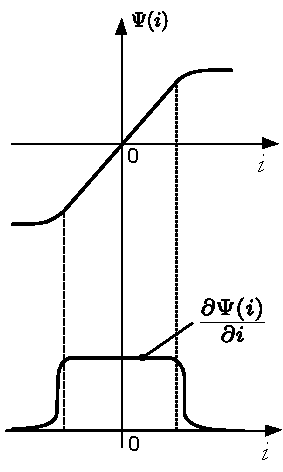
\includegraphics[width=0.5\linewidth]{mag_char_fer.pdf}
      \caption{Statická magnetizační charakteristika transformátoru s feromagnetickým jádrem a závislost   
               diferenciální indukčnosti na proudu.}
      \label{es:fig_mag_char_trafa_fer}
    \end{figure}            
    Dosadíme-li rov. \ref{es:eq_tok_proud} do rov. \ref{es_ind_u} a použijeme-li větu o derivaci
    složené funkce\footnote{Je-li $y = f(u), u = \varphi(x)$, potom derivace $y$ podle proměnné $x$
    je rovna derivaci $y$ podle proměnné $u$, násobené derivací $u$ podle proměnné $x$}, obdržíme
    pro napětí na cívce:
    \begin{equation}\label{es_tok_deriv}
      u(t) = \frac{d}{dt} f[i(t)] = \frac{\Psi(i)}{di} \frac{di}{dt} = L_d \cdot \frac{di}{dt}
    \end{equation}

    kde $L_d=\frac{d\Psi(i)}{di}$ má význam \textbf{diferenciální indukčnosti}. Ta může být ve speciálních 
    případech konstantní, ale ve většině reálných aplikací je funkcí proudu cívkou. Jako příklad uvedeme 
    transformátor s feromagnetickým jádrem. Zde je závislost spřaženého magnetického toku na proudu silně 
    nelineárně závislá, obr.\ref{es:fig_mag_char_trafa_fer}. Potom mluvíme o nelineárních magnetických 
    obvodech.
    
    Na obr. \ref{es:fig_mag_char_trafa_fer} je zobrazena \textbf{statická magnetizační charakteristika} a 
    její derivace, představující průběh diferenciální indukčnosti vinutí v závislosti na proudu. Vidíme, že 
    pro malé proudy je indukčnost největší s rostoucím proudem prudce klesá, nastane-li tzv. přesycení 
    magnetického obvodu transformátoru. Tomuto režimu se snažíme správným návrhem transformátoru vyhnout. 
    Velmi často se v technické praxi zavádí zjednodušení, při kterém se reálný magnetický obvod linearizuje - 
    diferenciální indukčnost je považována za konstantní (nezávislá na proudu cívkou). Mluvíme pak o 
    lineárních magnetických obvodech. Toto zjednodušení je použitelné pouze tehdy, pokud reálný magnetický 
    obvod (transformátor) provozujeme v určitých mezích magnetizačního proudu, kdy se skutečná indukčnost
    příliš nemění. Nelineární magnetizační charakteristika na obr. \ref{es:fig_mag_char_trafa_fer} se 
    linearizuje do podoby na obr. \ref{figure:mag_lin}.

    Závislost spřaženého magnetického toku na proudu cívkou je tedy lineární ($L=konst$) viz obr.
    \ref{figure:mag_lin}:
    \begin{equation}\label{es_tok_L}
      \Psi(t)=f[i(t)] = L \cdot i(t)
    \end{equation}
    
    \begin{figure}
      \centering
      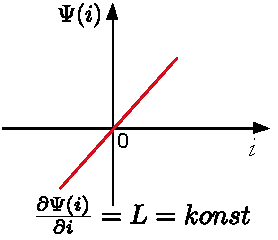
\includegraphics[width=0.7\linewidth]{mag_linearizace.pdf}
      \caption{Linearizovaná magnetizační charakteristika. Směrnice této přímky je právě rovna $L$}
      \label{figure:mag_lin}
    \end{figure}
    Dosazením spřaženého magnetického toku do Faradayova zákona elektromagnetické indukce - rov.
    \ref{es_ind_u}
    \begin{equation}\label{es_tok_faraday}
        u(t)=\frac{d}{dt}f[i(t)]=\frac{d}{dt}[L\cdot i]=L\cdot\frac{di}{dt}
    \end{equation}
    Ve zvláštním případě stejnosměrných veličin, kdy proud má lineární charakter, přejde vztah
    \ref{es_tok_L} do tvaru, který představuje tzv. \textbf{statickou definici indukčnosti}.
    \begin{equation}\label{es_stat_L}
      \Psi(t)= L \cdot I
    \end{equation}
    Je ale třeba zdůraznit, že rov. \ref{es_tok_L}, rov. \ref{es_tok_faraday} a rov. \ref{es_stat_L} 
    \emph{platí pouze pro lineární magnetické obvody}. Jestliže jsou použity při matematickém popisu 
    transformátorů nebo cívek s feromagnetickým jádrem, je třeba mít na paměti, že tento linearizovaný model 
    lze použít jen v určitém omezeném rozsahu daným skutečnou magnetizační charakteristikou. Nicméně, 
    lineární model transformátoru je pro svou jednoduchost často používán.
    
  %--------------------- Princip činnosti, základní konstrukční provedení ------------------------------------
  \section{Princip činnosti, základní konstrukční provedení}
    \begin{definition}
      \textbf{Transformátor} je elektrický netočivý stroj, který umožňuje pře\-nášet elektrickou energii z 
      jednoho obvodu do jiného pomocí vzá\-jemné elektromagnetické indukce. To znamená, že mění její 
      parametry (napětí, proudy), přitom forma energie na vstupu i výstupu zůstává elektrická.
    \end{definition}

    Transformátory jsou nezbytnou součástí řady elektrotechnických zařízení, počínaje vazebními a napájecími 
    transformátorky sdělovacích a polovodičových zařízení až k transformátorům blokovým a přenosovým, 
    užívaným v energetice. Jejich výkony se pohybují od zlomků VA do stovek MVA. Podobně je tomu s jejich 
    napětími od malých až po vvn. Zásadně transformátory  mohou být jedno nebo vícefázové (obvykle třífázové)

    \begin{figure}[ht!]
      \centering
      \subfloat[Schématická značka transformátoru s jádrem]{\label{enz:fig_trafo_core_sch}
        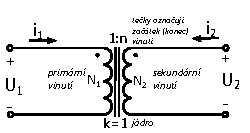
\includegraphics[width=0.9\linewidth]{SCH_Transformer_Core.pdf}}\newline
      \subfloat[Principiální provedení transformátoru se dvěma
                vinutími]{\label{es:fig_trafo_core_ideal}
        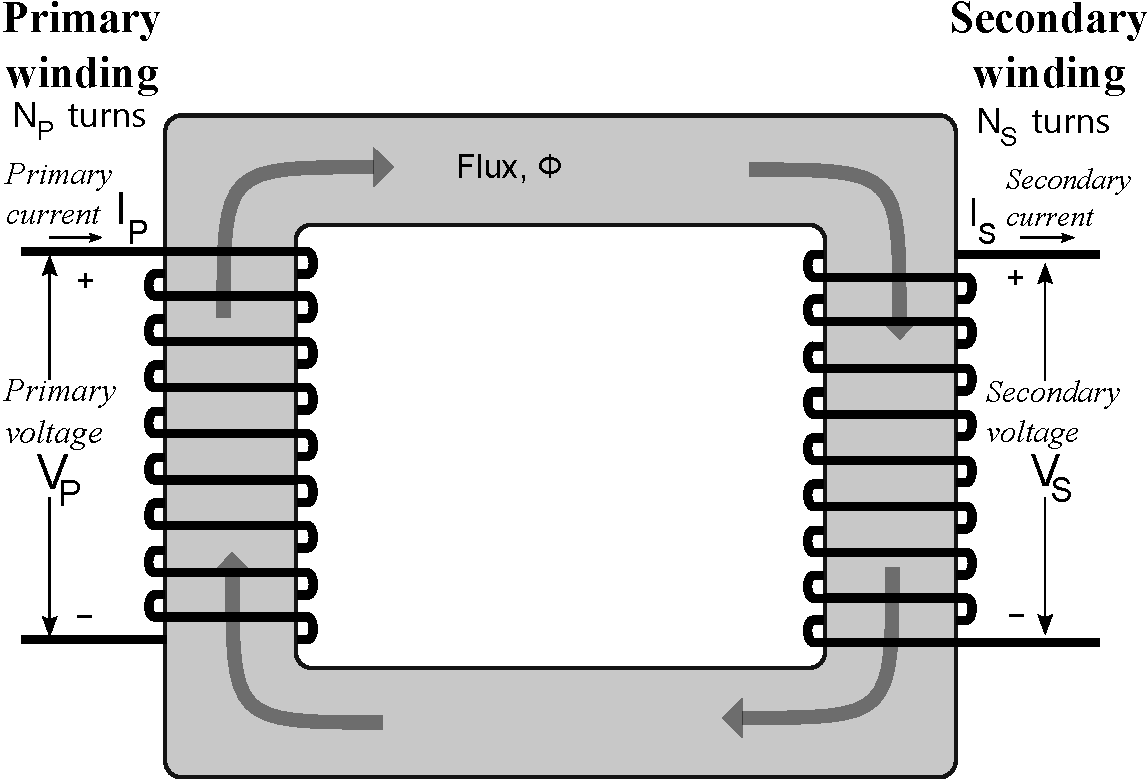
\includegraphics[width=0.9\linewidth]{wiki_single_phase_transformer.pdf}}
      \caption{Ideální transformátor s jádrem, s jedním primárním a jedním sekundárním 
               vinutím. Tečky označují začátky (resp. konce) vinutí. Význam má jejich poloha tečky vůči
               druhé. Budeme-li je chápat jako začátky vinutí, měl by se drát primáru a sekundáru
               vinout tak, jak je naznačeno na obrázku}
      \label{es:fig_trafo_ideal}
    \end{figure}
    Princip transformátoru je založen na \textbf{zákonu elektromagnetické indukce} - tedy magnetický tok 
    vybuzený jedním vinutím indukuje napětí ve vinutí druhém (primár, sekundár). Obrázek 
    \ref{es:fig_trafo_core_ideal} ukazuje, že magnetický tok je z jednoho vinutí do druhého veden     
    prostřednictvím magnetického obvodu. Fyzikální princip vychází z \textbf{2. Maxwellovy
    rovnice} \ref{es:eq_elmag_ind}.

    Převod transformátoru
    \begin{equation}\label{es:eq_turn_ratio}
        n = \frac{N_1}{N_2}; \quad n=\sqrt{\frac{L_1}{L_2}}
    \end{equation}
    
  %---------------- Zjednodušený rozbor funkce transformátoru --------------------------------------
  \section{Zjednodušený rozbor funkce transformátoru}\label{ES:kap_simple_rozbor_trafa}
    Uvažujme pro začátek transformátor s dokonale těsnou vazbou, tedy s \emph{činitelem vazby
    $k=1$, s nulovým rozptylovým magnetickým tokem a s konečnou velikostí indukčnosti $L_1$ a $L_2$
    primárního a sekundárního vinutí}

    \subsection{Situace při sekundárním vinutí naprázdno}\label{ES:kap_rozbor_trafa}
      %----------------------------------
      % image: patocka_balist_glvn.tex label: \label{es:fig_MJ_patocka_trf_naprzdn}
        %\documentclass{article}
%  \usepackage{circuitikz}

%\begin{document}
  \begin{wrapfigure}{r}{2.8in}
    \centering
	\begin{circuitikz} 
	  \draw
		(0,0) node[transformer] (T) {}
		node[ocirc] (A) at ([xshift=-1.5cm]T.A1) {}
		node[ocirc] (B) at ([xshift=-1.5cm]T.A2) {}
		node[ocirc] (C) at ([xshift=1.5cm]T.B1) {}
		node[ocirc] (D) at ([xshift=1.5cm]T.B2) {}
		node[circ]  (E) at ([xshift=0.4cm,yshift=-5pt]T.A1)  {}
		node[circ]  (F) at ([xshift=-0.4cm,yshift=-5pt]T.B1) {}
		(T.A1) to [-o] (A)
		(T.A2) to [-o] (B) 
		(T.B1) to [-o] (C)
		(T.B2) to [-o] (D)
		([yshift=+.25cm]T.west) node{$L_1$}
		([yshift=-.25cm]T.west) node{$N_1$}
	    ([yshift=+.25cm]T.east) node{$L_2$}
		([yshift=-.25cm]T.east) node{$N_2$} 
	  ;
	  \coordinate (X) at ([xshift=-0.6cm]B);
	  \draw (A) --+(-0.6,0) to [sV] (X) -- (B); 
		
	  \begin{scope}[shorten >= 10pt,shorten <= 10pt,]
		\draw[->] (A) -- node[right] {$u_1(t)$} (B); 
	  \end{scope}
		
	  \draw[->] ([xshift=-0.9cm,yshift=10pt]T.A1) -- node[above] {$i_1(t) = i_\mu(t)$} +(20pt,0);
	\end{circuitikz}	 
	\caption[Transformátor naprázdno.]{Transformátor naprázdno.}
    \label{es:fig_MJ_patocka_trf_naprzdn}
    \vspace*{-1\baselineskip}
  \end{wrapfigure} 
%\end{document}  
      %----------------------------------
      Podle indukčního zákona platí pro primární a sekundární napětí
      \begin{subequations}
        \begin{align}
          u_1(t)=\frac{d\Psi_\mu}{dt} = N_1\frac{d\Phi_\mu}{dt}\label{es_eq_trafo1} \\
          u_2(t)=\frac{d\Psi_\mu}{dt} = N_2\frac{d\Phi_\mu}{dt}\label{es_eq_trafo2}
        \end{align}
      \end{subequations}      
      kde $\Phi_\mu(t)$ je magnetický tok v jádře. Porovnáním rov. \ref{es_eq_trafo1} a rov. 
      \ref{es_eq_trafo2} dostaneme následující rovnici:
      \begin{equation}\label{es_int_uprim_trafo}
          u_2(t)=u_1(t)\frac{N_2}{N_1}
      \end{equation}

      Je zřejmé, že $u_1(t)$ a  $u_2(t)$ mohou mít sice různou velikost, ale mají zcela stejný časový průběh. 
      Z rov. \ref{es_eq_trafo1} plyne, že magnetický tok je jednoznačně určen časovým integrálem z 
      přiloženého primárního napětí:
      \begin{equation}\label{es_eq_int_uprim}
          \Phi_\mu(t)=\frac{\int u_1(t)dt}{N_1}+\Phi_{\mu_{poc}}
      \end{equation}
      Primární napětí musí mít nulovou střední hodnotu, tj. nesmí mít stejnosměrnou složku, jinak by 
      magnetický tok rostl nade všechny meze (v praxi do přesycení). Velikost integrační konstanty 
      $\Phi_{\mu_{poc}}$ závisí na konkrétním režimu transformátoru. Z rovnice také plyne užitečný vztah:
      \begin{equation}\label{es_eq_int_uprim_max}
          \Delta\Phi_\mu(t)=\frac{\max|\int u_1(t)dt|}{N_1}
      \end{equation}
      Je-li $u_1(t)$ periodická funkce s nulovou střední hodnotou, pak neurčitý integrál z $u_1(t)$
      je rovněž periodická funkce, jejíž střední hodnota již ovšem nulová být nemusí (viz obr.
      \ref{es:fig_trafo_int_uprim}). $\Phi_\mu$ je rozkmit magnetického toku v jádře transformátoru.
      Z rovnice \ref{es_eq_int_uprim} je patrné, že bez bližší znalosti režimu transformátoru sice nelze 
      přesně stanovit meze, v nichž se magnetický tok periodicky pohybuje, ale dle rov.       
      \ref{es_eq_int_uprim_max} umíme přesně stanovit rozkmit toku čili vzdálenost mezí. Pro předpokládané 
      homogenní rozložení pole ve feromagnetickém jádře lze určit rozkmit magnetické indukce:
      \begin{equation}\label{es_eq_rozkmit_B}
        \Delta B_\mu(t)=\frac{\Delta\Phi_\mu(t)}{S}=\frac{\max|\int u_1(t)dt|}{N_1S}
      \end{equation}

      \begin{figure}[ht!]
        \centering
        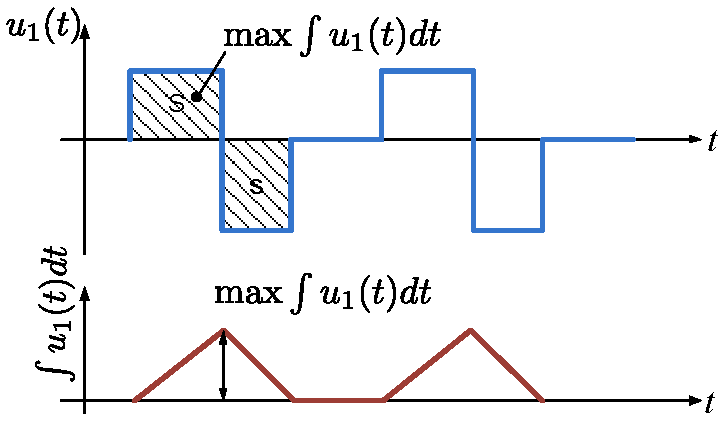
\includegraphics[scale=0.8]{trafo_int_uprim.pdf}
        \caption{Znázornění časového integrálu primárního napětí transformátoru.}
        \label{es:fig_trafo_int_uprim}
      \end{figure}

      pro \emph{lineární} magnetické obvody vztah mezi tokem a magnetizačním proudem:
      \begin{equation}\label{es_eq_stat_def_L}
        N_1\Phi_\mu(t)=L_1i_\mu(t)
      \end{equation}
      Proud $i_\mu(t)$ je primární proud při sekundárním vinutí naprázdno, tzv. \textbf{magnetizační proud}. 
      Je tedy přímo úměrný magnetickému toku $\Phi_\mu(t)$.
      \begin{equation}\label{es_eq_imag}
        i_\mu(t)=\frac{N_1\Phi_\mu(t)}{L_1}
      \end{equation}
      Dosadíme-li za $\Phi_\mu(t)$ rov. \ref{es_eq_int_uprim} uvedené na stránce \pageref{es_eq_int_uprim}, 
      dostaneme známý vztah mezi proudem a napětím cívky, vyjádřený v
      integrálním tvaru:
      \begin{equation}\label{es_eq_imag_u1}
        i_\mu(t)=i_{\mu_{poc}}+\frac{1}{L_1}\int{u_1(t)dt}
      \end{equation}
      Opět vidíme, že primární napětí musí mít nulovou střední hodnotu.
      
    %-------------------------------------- Situace při zatížení sekundárního vinutí -------------------------
    \subsection{Situace při zatížení sekundárního vinutí}
      Rovnice \ref{es_int_uprim_trafo} až rov. \ref{es_eq_imag_u1} zůstávají v platnosti. Připojíme-li k 
      sekundárnímu vinutí zátěž, začne téci sekundární proud $i_2(t)$. Např. pro odporovou zátěž bude platit

      \begin{equation}\label{es:eq_i2}
        i_2(t)=\frac{u_2(t)}{R_2}
      \end{equation}

      Se sekundárním proudem je svázán magnetický tok $\Phi_2(t)$
      \begin{equation}\label{es:eq_tok_phi2}
        \Phi_2(t)=\frac{L_2i_2(t)}{N_2}
      \end{equation}
      %----------------------------------
      % image: MJ_patocka_trf_Rz.tex label: \label{es:fig_MJ_patocka_trf_Rz}
      %  \documentclass{article}
  \usepackage{circuitikz}  
  \usepackage{wrapfig}
  
\begin{document}
  \begin{wrapfigure}[10]{r}{2.5in}
    \centering
	\begin{circuitikz} 
  	  \draw
	    (0,0) node[transformer] (T) {}
	node[ocirc] (A) at ([xshift=-1.5cm]T.A1) {}
	node[ocirc] (B) at ([xshift=-1.5cm]T.A2) {}
	node[ocirc] (C) at ([xshift=1.5cm]T.B1) {}
	node[ocirc] (D) at ([xshift=1.5cm]T.B2) {}
	node[circ]  (E) at ([xshift=0.4cm,yshift=-5pt]T.A1) {}
	node[circ]  (F) at ([xshift=-0.4cm,yshift=-5pt]T.B1) {}
	(T.A1) to [-o] (A)
	(T.A2) to [-o] (B) 
	(T.B1) to [-o] (C)
	(T.B2) to [-o] (D)
	([yshift=+.25cm]T.west) node{$L_1$}
	([yshift=-.25cm]T.west) node{$N_1$}
    ([yshift=+.25cm]T.east) node{$L_2$}
	([yshift=-.25cm]T.east) node{$N_2$} 
	;
	\coordinate (X) at ([xshift=-0.6cm]B);
	\coordinate (Y) at ([xshift=+0.6cm]D);
	\draw       (A) --+(-0.6,0) to [sV] (X) -- (B); 
	\draw       (C) --+(0.6,0)  to [R]  (Y) -- (D); 
	
	\begin{scope}[shorten >= 10pt,shorten <= 10pt,]
	  \draw[->] (A) -- node[right] {$u_1(t)$} (B); 
	  \draw[->] (C) -- node[left] {$u_2(t)$} (D);
	\end{scope}
	
	\draw[->] ([xshift=-0.9cm,yshift=10pt]T.A1) -- node[above]
	          {$i_1(t) = i_\mu(t)+i_1'(t)$} +(20pt,0);
	\draw[<-] ([xshift=0.9cm,yshift=10pt]T.B1)  -- node[above] 
	          {$i_2(t)$} +(-20pt,0);
	\end{circuitikz}	 
	\caption[Transformátor zatížený]{Transformátor zatížený}
    \label{es:fig_MJ_patocka_trf_Rz}
  \end{wrapfigure} 
\end{document}  
      %----------------------------------
    
      \begin{wrapfigure}{r}{2.3in}
        \centering
        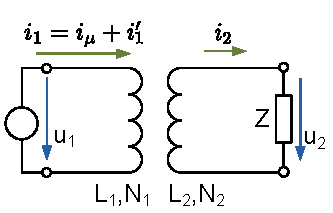
\includegraphics[scale=1]{trafo_zatizeny.pdf}
        \caption{Transformátor zatížený.}
        \label{es:fig_trafo_zatizeny}
        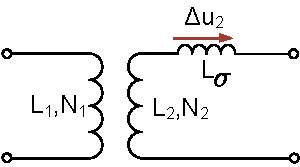
\includegraphics[scale=1]{patocka_trafo_rozptyl.pdf}
        \caption{Zjednodušená představa rozptylu reálného transformátoru.}
        \label{es:fig_trafo_rozptyl}
      \end{wrapfigure}
      Proud $i_2(t)$, tedy i tok $\Phi_2(t)$, mohou mít bohužel stejnosměrnou složku (zátěží může být např. 
      jednocestný usměrňovač). Stejno\-směr\-nou složku prou\-du však transformátor obecně neumí 
      pře\-trans\-form\-ovat na primární stranu a pak do\-chází ke stejnosměrné před\-magnet\-izaci jádra 
      (sekundární proud stejno\-směr\-nou složku obsahuje, primární proud nikoli). Jedná se o škodlivý jev, 
      který může způsobit, zvláště při větších proudech i přesycení magnetického obvodu. Jev nastává např. 
      při napájení transformátoru ze sítě. Síť se totiž jeví v průběhu celé pracovní periody jako napěťový 
      zdroj s malou vnitřní impedancí. Za zvláštních okolností transformátor stejnosměrnou složku 
      transformovat umí, např. v jednočinném propustném měniči. Zde je transformátor po určitou část periody 
      od primárního zdroje odpojen, v té chvíli se vnitřní impedance primárního zdroje jeví jako nekonečně 
      velká. Oba typy napájení je nutno rozlišovat.

      Dále proto uvažujeme pouze takové typy zátěží, které stejnosměrnou složku ne\-vy\-tvá\-ře\-jí      
      (např. zátěž typu dvoucestný můstkový usměrňovač již tuto nectnost nemá). Pak při uvažování dokonalé 
      vazby, tj. při činiteli vazby $k=1$, je v celém magnetickém obvodu sekundární tok $\Phi_2(t)$ plně 
      vykompenzován primárním tokem $\Phi_1(t)$ stejné velikosti, ale opačného znaménka. Tok $\Phi_1(t)$ je 
      svázán s "přídavným" primárním proudem, tedy proudem pře\-trans\-formovaným ze sekundáru na primár - 
      nazvaný jako $i_1'(t)$. Proud vzniká v primárním vinutí v důsledku Lenzova pravidla. Je zodpovědný za 
      čerpání energie z primárního napájecího zdroje a jeho existence je současně v souladu se zákonem 
      zachování energie

      \begin{equation}\label{es:eq_zachovani_energie}
        \Phi_1(t)=\frac{L_1i_1'}{N_1}=\Phi_2(t)
      \end{equation}

      Srovnáním rov. \ref{es:eq_tok_phi2} a rov. \ref{es:eq_zachovani_energie} obdržíme známý vztah
      pro transformaci proudů:
      \begin{equation}\label{es:eq_i1_cark}
        i_1'(t)=i_2(t)\frac{L_2N_1}{N_2L_1}=i_2 (t)\frac{N_2^2N_1}{N_2N_1^2}=i_2(t)\frac{N_2}{N_1}
      \end{equation}
      Celkový primární proud $i_1(t)$ tedy při zatížení transformátoru sestává ze dvou zcela nezávislých 
      složek. Jednou složkou je magnetizační proud $i_\mu(t)$, který tekl už i ve stavu naprázdno (a nyní při 
      zatížení se nezměnil) a druhou je výše zmiňovaný přetransformovaný proud $i_1'(t)$ :
      \begin{equation}\label{es:eq_i1_sum}
        i_1(t)=i_1'(t)+i_\mu(t)
      \end{equation}
      Z dosud uvedených skutečnosti plyne důležitý závěr: tok v jádře zůstává nezměněn i při zatížení, je 
      tedy stále roven původnímu toku $\Phi_\mu(t)$, protože tok $\Phi_1(t)$ od proudu $i_1'(t)$ a tok 
      $\Phi_2(t)$ od proudu $i_2(t)$ se plně kompenzují. \emph{Sycení jádra u \textbf{bezrozptylového} 
      transformátoru tedy vůbec nezávisí na velikosti zatěžovacího prou\-du, tedy ani na velikosti 
      přenášeného výkonu!}

      Reálné transformátory mají vždy určitý \emph{rozptylový tok}. Ten je svázán s tzv.      
      roz\-pty\-lo\-vý\-mi indukčnostmi (primární a sekundární): Takový transformátor si můžeme představit 
      jako transformátor bezrozptylový s připojen\-ými indukčnostmi $L_{\sigma1}$ do série s pri\-már\-ním 
      vinutím a $L_{\sigma2}$ do série se sekundár\-ním vinutím. Z hlediska vnějšího chování transformátoru 
      lze uvažovat i jedinou rozptylovou indukčnost $L_\sigma$, přepočtenou jen na sekundární stranu (viz 
      obr. \ref{es:fig_trafo_rozptyl}).

      Tento tok je samozřejmě svázán s úbytkem sekundárního napětí $\Delta u_2(t)$ na $L_\sigma$.
      Čili \emph{rozptylová indukčnost způsobuje nenulovou výstupní reaktanci transformátoru},
      Transformátor je pak "\emph{měkký}", zatěžovací proud způsobí úbytek napětí:
      \begin{equation}\label{es:eq_ubytek_Lsigma}
        u_2(t)=N_2\frac{d\Phi_\sigma(t)}{dt}
      \end{equation}
      Skutečný transformátor má navíc nenulové odpory vodičů, na kterých vznikají podle Ohmova
      zákona další úbytky napětí a navíc Joulovy ztráty.

      Vraťme se nyní znovu k transformátoru bezrozptylovému, s dokonalou vazbou, a předpokládejme, že jeho 
      vinutí mají navíc nulový odpor (supravodič). Pak na nich nevzniká průchodem proudu žádný ztrátový výkon 
      a proudy $i_2(t)$  a $i_1'(t)$ lze libovolně zvyšovat. Jejich magnetické účinky se dokonale zruší, 
      nemají tedy vliv na velikost sycení v jádře a transformátorem lze přenášet "libovolně" velký výkon (ve 
      skutečnosti však omezený tzv. kritickou proudovou hustotou supravodiče, při níž zaniká supravodivý jev 
      - pro niob asi 50 A/mm2).

      U měděného (hliníkového) vinutí je nutno volit průřez vodičů úměrný proudu, aby nebyla překročena 
      dovolená proudová hustota s ohledem na přehřátí vodičů vlivem Joulova tepla. Rovnice 
      \ref{es_eq_rozkmit_B} navíc napovídá, že musíme volit určitý počet primárních závitů $N_1$, abychom 
      nepřekročili maximální sycení jádra. $N_1$ je tím větší, čím je větší maximum - amplituda časového 
      integrálu primárního napětí a čím menší průřez má jádro. Má-li se pak vinutí vtěsnat do okénka jádra, 
      nelze zvyšovat průřez vodiče a tím i proudovou zatížitelnost libovolně. Díky tomu lze s daným průřezem 
      magnetického obvodu $S$ a průřezem okénka $S_0$ realizovat transformátor schopný přenést jen určitý 
      omezený výkon.

      Je tedy zřejmé, že maximální výkon bude přímo úměrný ploše okénka $S_0$, protože čím je $S_0$ větší, 
      tím tlustší vodiče můžeme použít a tím větší proudy (výkon) je možno transformovat. Kromě toho je 
      maximální výkon přímo úměrný i průřezu magnetického obvodu $S$, protože čím je $S$ větší, tím méně 
      závitů $N_1$ potřebujeme pro dané sycení, viz rov. \ref{es_eq_rozkmit_B}, a proto mohou být opět 
      tlustší vodiče. Čili lze napsat:
      \begin{equation}\label{es:eq_Pmax}
        P_{max} \approx S\cdot S_0
      \end{equation}

      Zamyslíme-li se nad rov. \ref{es_eq_rozkmit_B}, lze úměru rov. \ref{es:eq_Pmax} ještě doplnit. 
      Maximální hodnota sycení tj. maximum funkce $B(t)$ je přímo úměrná maximu funkce časového integrálu 
      primárního napětí. Uvažujme, že napětí neobsahuje stejnosměrnou složku, je periodické s kmitočtem $f$, 
      ale jinak libovolného tvaru, tj. libovolného obsahu vyšších harmonických.

      Pak je maximum časového integrálu takového primárního napětí (maximum toku, amplituda toku) zcela jistě 
      konečné a nepřímo úměrné kmitočtu. To znamená, že zvýšíme-li kmitočet n-krát při zachování amplitudy a 
      tvaru napětí, klesne maximum integrálu n-krát a bude moci být dle rov. \ref{es_eq_rozkmit_B} také 
      n-krát méně závitů $N_1$, aby sycení zůstalo stejné. Pak ve stejném poměru n můžeme zvýšit průřez 
      vodičů, aniž bychom se báli, že se vinutí nevejde do okénka. Lze pak přenášet n-krát větší proud a 
      výkon (napětí se nezměnila, pouze vzrostl kmitočet). Čili maximální výkon je přímo úměrný kmitočtu. 
      Rovnici \ref{es:eq_Pmax} lze proto doplnit:
      \begin{equation}\label{es:eq_Pmax2}
        P_{max} \approx f\cdot S\cdot S_0
      \end{equation}
      Pro jádra z plechu EI z křemíkové oceli lze pomocí tohoto vztahu s uvažováním přímé úměry mezi $S_0$ a 
      $S$, odvodit vztah
      \begin{equation}\label{es:eq_Pmax_EI}
        P_{max} \approx S^2\quad [W, cm^2]
      \end{equation}
      Ten předpokládá maximální sycení $1 T$, proudovou hustotu asi $2,5 A/mm^2$ a kmitočet $50 Hz$. A týká 
      se opravdu jen EI jader, protože při jeho odvození byla uvažována konkrétní závislost mezi $S_0$ a $S$ 
      pro tato jádra.

      Ze vztahu rov. \ref{es:eq_Pmax2} vidíme, že zvyšování pracovního kmitočtu umožňuje přenášet větší výkon 
      při zachování rozměrů jádra. To je základem filosofie všech spínaných zdrojů (měničů) s 
      transformátorem. Kmitočet však nelze u reálného transformátoru zvyšovat nade všechny meze. Omezení 
      představují hysterezní a vířivé ztráty v jádře a dále rozptylová indukčnost.

  \section{Ztráty v reálném transformátoru}
    \subsection{Joulovy ztráty ve vinutí}
      Joulovy (ohmické) ztráty vznikají na odporu vinutí průchodem proudu. Tato sku\-te\-čnost nutí zvyšovat 
      průřez vodičů a způsobuje tak nutné zvyšování plochy okénka jádra $S_0$ a zvětšování celého 
      transformátoru.

      Z hlediska těchto ztrát se primární a sekundární vinutí chovají jako lineární odpory $R_1$ a $R_2$. 
      Joulovy ztráty jsou proto úměrné kvadrátu efektivní hodnoty procházejícího proudu a jsou dány vztahem:
      \begin{equation}\label{es_joul_loss}
        P_R= R_1 I_{1_ef}^2 + R_2 I_{2_ef}^2
      \end{equation}

      Efektivní hodnota proudů procházejících vinutími obecně není úměrná přenášenému činnému výkonu a může 
      být v praxi někdy nečekaně vysoká. Např. u síťového transformátoru se sekundárním usměrňovačem a 
      filtračním kondenzátorem bez vyrovnávací nárazové tlumivky. Zde odebíraný sekundární proud $i_2(t)$ a 
      tedy přetransformovaná složka primárního proudu $i_1'(t)$ tvar úzkých nabíjecích impulsů s velkou 
      amplitudou. Jeho celková efektivní hodnota je několikrát větší než efektivního hodnota užitečné 1. 
      harmonické, která se v tomto případě pouze samotná podílí na přenosu činného výkonu. Ten je totiž dán 
      součinem efektivní hodnoty harmonického sekundárního napětí, efektivní hodnoty pouze 1. harmonické 
      sekundárního proudu a $\cos\phi$ oné 1. harmonické proudu!

      Pro omezení ohřevu vinutí na přípustnou mez je nutno omezit odpory vinutí. Při návrhu pracujeme s tzv. 
      dovolenou proudovou hustotou $J$. Teče-li proud rovno\-měr\-ně celou plochou průřezu vodiče, platí 
      vztahy:
      \begin{equation}\label{es_proud_hustota}
        J_1=\frac{I_{1_{ef}}}{S_1} \quad J_2=\frac{I_{2_{ef}}}{S_2}
      \end{equation}
      $S_1$ a $S_2$ jsou průřezy primárního  a sekundárního vinutí.

      Doporučená hodnota $J$ se pohybuje v případě měděných vodičů v rozmezí $1,5$ až $7 A/mm^2$. Pro větší 
      transformátory s velkým objemem vinutí je třeba volit vždy hustotu menší. Při \emph{konstantní proudové 
      hustotě totiž celkový Joulův ztrátový výkon roste s třetí mocninou lineárních rozměrů cívky, chladící 
      povrch pouze s druhou mocninou}. Vinutí těsně pod chladícím povrchem mohou mít větší proudovou hustotu 
      než vinutí vnitřní.

      Bez nuceného proudění vzduchu volíme u toroidních transformátorů hustotu $J$ v rozsahu $2$ až
      $5 A/mm^2$, podle velikosti a počtu vrstev vinutí. U malých hrníčkových feritových jader lze volit 
      nouzově až $4,5 A/mm^2$. U běžně užívaných síťových transformátorů s mnohovrstvými cívkami vinutými na 
      kostrách se doporučuje hodnota $1,5 A/mm^2$ (pro velké transformátory) až $3,5 A/mm^2$ (pro malé 
      transformátorky). Při použití nuceného proudění vzduchu může být hustota $J$ větší.

      U transformátorů pracujících na vysokém kmitočtu musíme počítat s uplatněním \textbf{skinefektu}, díky 
      němuž proud teče jen ve vrstvě pod povrchem vodiče a střední část tlustého vodiče by tak byla nevyužita.

    \subsection{Hysterezní ztráty v jádře}
      Hysterezní ztráty souvisejí s energií $W$ potřebnou na přemagnetování jádra. Energie $W$ je úměrná 
      ploše hysterezní smyčky (viz. obr. 3.5). Plocha hysterezní smyčky má fyzikální rozměr $J/m^3$, jedná se 
      tedy o objemovou hustotu ztrátové energie. Ta je pak  velká pro materiály magneticky tvrdé, se širokou 
      hysterezní smyčkou tj. s velkou \emph{remanencí} $B_R$ a \emph{koercitivní intenzitou} $H_C$. Takové 
      materiály proto nejsou pro jádra transformátoru vhodná. Naopak požadujeme materiály magneticky měkké, s 
      co nejužší hysterezní smyčkou a s co nejmenší remanentní indukcí.

      Je zřejmé, že velikost plochy hysterezní smyčky $S$ a tedy i energie $W$ souvisí nejen s vlastnostmi 
      materiálu $B_R$ a $H_C$, ale i s amplitudou indukce $B_m$. Přibližně platí, že plocha $S$ je úměrná 
      kvadrátu $B_m$.(viz. obr. 3.5). Hysterezní ztrátový výkon je dán součinem této energie $W$ a pracovního 
      kmitočtu $f$, v jehož „rytmu“ dochází k přemagnetovávání.

      \begin{equation}\label{ES:eq_hyster_loss}
        P_h = W \cdot f \approx B_m^2 \cdot f^2
      \end{equation}

      \begin{figure}[ht!]
        \centering
        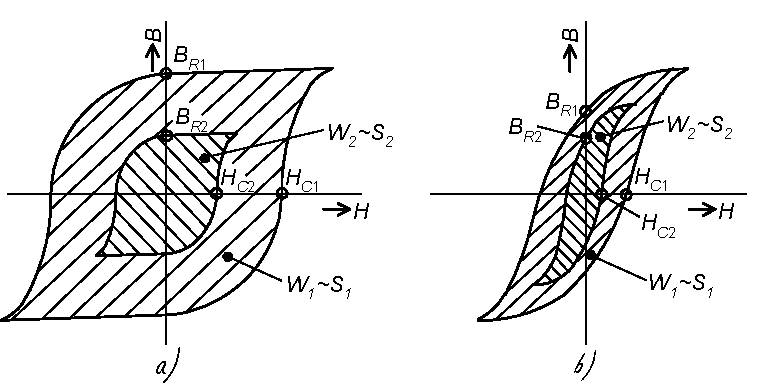
\includegraphics[width=1\linewidth]{patocka_BH_curve.pdf}
        \caption[Hysterezní smyčka feromagnetického materiálu]{Hysterezní smyčka feromagnetického
                 materiálu: \newline a) magneticky tvrdý materiál, \newline b) magneticky měkký
                 materiál.}
        \label{es:fig_BH_curve}
      \end{figure}

      \begin{itemize}
        \item Budeme-li měnit kmitočet a současně zachovávat sycení, tzn. budeme udržovat konstantní poměr 
              amplitudy  $u_1(t)$ a kmitočtu $f$ při proměnném počtu závitů  $N_1$ – viz rozbor vztahu 
              (\ref{es_eq_rozkmit_B}). Pak bude díky konstantnímu sycení $B_m$ i konstantní energie $W$. Ze 
              vztahu (\ref{ES:eq_hyster_loss}) je pak vidět, že hysterezní ztráty budou přímo úměrné kmitočtu.
              \begin{equation}\label{ES:eq_hyst_loss_linf}
                P_h \approx f
              \end{equation}
              Toto je typický případ transformátoru v pulsních měničích, kdy volíme vysoký kmitočet za účelem 
              snížení  $N_1$ (aby se vinutí mohlo vinout tlustším vodičem) při zachování (nepřekročení) 
              dovoleného sycení.
        \item Měníme-li kmitočet a současně zachovávat týž transformátor (totéž $N_1$ a $S$) a tutéž 
              amplitudu $u_1(t)$. Pak z rozboru vztahu (\ref{es_eq_rozkmit_B}) vyplývá, že indukce bude 
              nepřímo úměrná kmitočtu.  Čili ze vztahu (\ref{ES:eq_hyster_loss}) pak vidíme, že hysterezní 
              ztráty budou \emph{hyperbolicky}, nepřímo úměrně, klesat s rostoucím kmitočtem.
              \begin{equation}\label{ES:eq_hyst_loss_hypf}
                P_h \approx \frac{1}{f}
              \end{equation}
              Tento režim transformátoru se nazývá \emph{odbuzovací}, neboť při růstu kmitočtu klesá indukce. 
              V pulsních měničích by ale takový režim neměl žádný význam, protože bychom sice zvýšili 
              kmitočet, ale museli bychom použít stále stejný objemný a těžký transformátor s velkým $N_1$, 
              stanoveným pro původní nízký kmitočet.
      \end{itemize}

    \subsection{Ztráty vířivými proudy v jádře}
  \section{Rozptyl transformátoru}
    Vraťme se nyní k zjednodušenému modelu rozptylu z obr. \ref{es:fig_trafo_rozptyl}. Pro velikost
    roz\-ptyl\-ové indukčnosti $L_\sigma$ platí:
    \begin{equation}\label{es:eq_Lsigma}
      L_\sigma=\lambda_\sigma\cdot N_2^2
    \end{equation}
    kde $\lambda_\sigma$ je \emph{magnetická vodivost rozptylového magnetického obvodu}. Rozptylovou 
    indukčnost $L_\sigma$ (tj. sekundární rozptylovou indukčnost plus primární rozptylovou indukčnost 
    přepočtenou na sekundární stranu) je nutno chápat jako indukčnost určující výstupní reaktanci 
    transformátoru napájeného ovšem z ideálního napěťového primárního zdroje. Lze ji snadno změřit, 
    zkratujeme-li primární vinutí a měříme sekundární indukčnost
    $L_{2,k}$:
    \begin{equation}\label{es:eq_L2k}
      L_\sigma=L_{2,k}= L_2(1-k^2)
    \end{equation}
    kde $k$ má význam \emph{činitele vazby} a lze jej určit ze známého vztahu:
    \begin{equation}\label{es:eq_cinitel_vazby}
      k=\frac{M}{L_1L_2}
    \end{equation}
    Zajímá nás ovšem \textbf{výstupní reaktance} $\omega L_\sigma$, nikoliv samotná indukčnost $L_\sigma$, 
    neboť napěťový úbytek je úměrný (při harmonickém průběhu napětí):
    \begin{equation}\label{es:eq_nap_ubytek}
      \Delta u_2(t)\approx \omega L_\sigma
    \end{equation}
    Je zřejmé, že při konstantní rozptylové indukčnosti může být transformátor na vysokých kmitočtech 
    naprosto nepoužitelný (měkký). Pak nezbývá, než velmi ú\-zkost\-li\-vě a co nejvíce minimalizovat 
    rozptylovou indukčnost. Je proto nutné podle rov. \ref{es:eq_Lsigma} minimalizovat rozptylovou 
    magnetickou vodivost $\lambda_\sigma$. Ta je přibližně určená rovnicí:
    \begin{equation}\label{es:eq_rozptyl_vodivost}
      \lambda_\sigma= \mu_0\frac{S_\sigma}{l_\sigma}
    \end{equation}
    kde $\mu_0=4\cdot\pi10^{-7}H/m$ je \emph{permeabilita vakua}. $S_\sigma$ a $l_\sigma$ jsou
    \textbf{ekvivalentní průřez} a \textbf{délka rozptylových cest}. Protože nelze snížit  permeabilitu 
    vzduchu, je nutno upravit geometrii jádra a současně zabezpečit co největší poměr permeability jádra k 
    permeabilitě okolního prostředí. Jádro musí mít tvar bez ostrých zlomů ve směru magnetického toku, 
    nejlépe kruhový tvar, tj. \emph{toroidní jádro}. Je důležitá velká magnetická vodivost jádra $\lambda$. 
    Ta je dána vztahem:
    \begin{equation}\label{es:eq_vodivost_jadra}
      \lambda= \mu_r\mu_0\frac{S}{l}
    \end{equation}
    $\mu_r$ je \emph{relativní permeabilita materiálu}, $S$ je \emph{průřez jádra}, $l$ je \emph{délka 
    střední siločáry}. Nestačí jen velká permeabilita  $\mu_r$, ale i velký poměr $\frac{S}{l}$. Pro 
    minimalizaci rozptylu jsou proto vhodná "baculatější" jádra s velkým $S$ a malým $l$ (často například 
    několik toroidů s malým průměrem tj. malým $l$ paralelně pro dosažení velkého $S$). Tím ale vzniká 
    problém malého okénka $S_0$ pro vinutí, což znemožňuje vinout vodiči s velkým průřezem a přenášet tak 
    velké výkony. Tyto protichůdné požadavky na tvar jádra bývají kritické a je nutno je v návrhu kompromisně 
    vyřešit.

    Rozptylovou indukčnost dále zmenšíme způsobem vinutí. Jsou-li vinutí na kostřičce, pak je vineme na sebe, 
    nikoliv vedle sebe s přepážkou. Blíže jádru umístíme vinutí s menším počtem závitů. Vhodné je také 
    střídavé prokládání jednotlivých vrstev primárního a sekundárního vinutí, roste však neúměrně pracnost 
    (cena) a klesá činitel plnění okénka. \emph{Bifilární vinutí} s nejtěsnější vazbou nelze uskutečnit v 
    případě rozdílných počtů závitů (což je téměř vždy) a v případě nároků na izolační pevnost mezi vinutími 
    rozprostřenými rovnoměrně po obvodu celého toroidu.

    \subsection*{Poznámka k transformátorům obecně (nejen síťovým)}
      Všimněme si, že v celém výkladu není nikde zmínka o použití \emph{vzduchové mezery v magnetickém obvodu 
      jádra}. V kapitole Cívky s feromagnetickým jádrem je zamyšlení o vzduchových mezerách v magnetických 
      obvodech a je zde vysvětlen jediný případ, kdy má smysl mezeru v transformátoru použít. Je zde ukázáno, 
      že v případě předpokladu platnosti rov. \ref{es_eq_int_uprim_max} (což je mimo jiné případ běžných 
      napájecích transformátorů) je použití vzduchové mezery bezúčelné a škodlivé, vede totiž ke vzrůstu 
      magnetizačního proudu a zvýšení rozptylových toků.

  \section{Cívky s feromagnetickým jádrem}
    \subsection{Fyzikální rozbor a příprava pro návrh}
    \subsection{Důsledky a význam použití vzduchové mezery}
    
  \newpage
  \section{Efektivní hodnoty proudů typických prů\-bě\-hů}
    Pro správnou volbu průřezu drátu pro vinutí je nutné stanovit přípustné oteplení, které je určeno 
    efektivní hodnotou proudu. Pro nejčastější průběhy proudů jsem odvodil vztahy pro výpočet efektivních 
    hodnot.
    \begin{figure}[b]
      \centering
      \subfloat[$I_{ef}=I_{max}\sqrt{\frac{\delta}{3}}$]{\label{es:fig_current_ef_solve_1}
         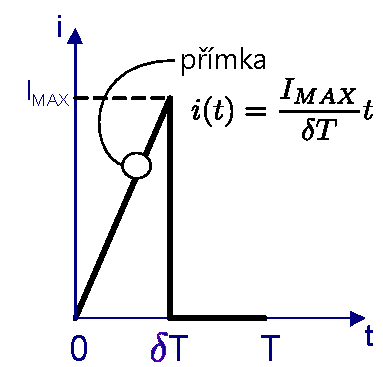
\includegraphics[width=0.3\linewidth]{current_ef_solve_1.pdf}}
      \subfloat[$I_{ef}=I_{max}\sqrt{\frac{1}{3}}$]{\label{es:fig_current_ef_solve_2}
         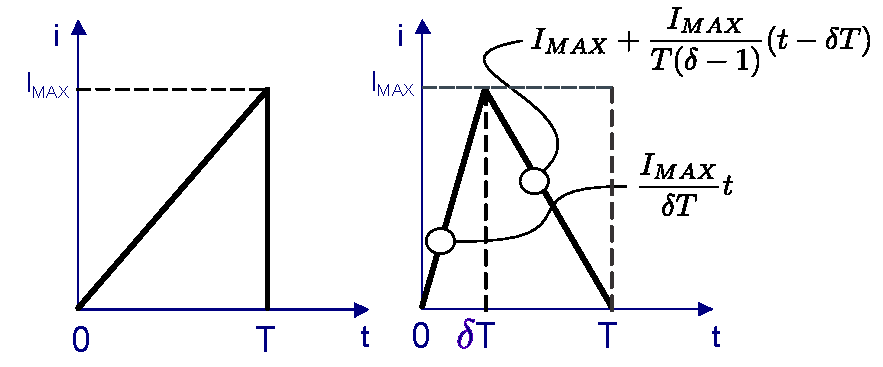
\includegraphics[width=0.6\linewidth]{current_ef_solve_2.pdf}}
      \caption{Typické průběhy proudů, jejichž efektivní hodnotu je nutné stanovit při dimenzování
               vinutých komponent.}
      \label{es:fig_Ief_solve1}
    \end{figure}

    \begin{enumerate}
      % ===========================================================================================
      \item Výpočet efektivní hodnoty proudu s průběhem na obrázku \ref{es:fig_current_ef_solve_1}:
        \begin{align}\label{es:eq_Ief1_solve}
          I_{ef}^2 &=  \frac{1}{T}\int_0^{\delta T}i^2(t)dt=
                       \frac{1}{T}\int_0^{\delta T}
                                         {\left(\frac{I_{max}}{\delta T}t\right)^2}dt   \\ \nonumber
                   &=  \frac{1}{T}\left(\frac{I_{max}}{\delta T}\right)^2
                       \int_0^{\delta T}{t^2}dt =
                       \frac{1}{T}\left(\frac{I_{max}}{\delta T}\right)^2
                                  \left[\frac{t^3}{3}\right]_0^{\delta T}               \\ \nonumber
                   &=  \frac{1}{T}\frac{I_{max}^2}{(\delta T)^2}
                       \frac{(\delta T)^3}{3}=I_{max}^2\frac{\delta}{3}
        \end{align}

      % ===========================================================================================
      \item Výpočet efektivní hodnoty proudu s průběhem na obrázku \ref{es:fig_current_ef_solve_2}:
            Pravý průběh na obrázku \ref{es:fig_current_ef_solve_2} je speciálním případem levého
            průběhu jehož efektivní hodnotu snadno určíme jako $I_{max}\sqrt{\frac{1}{3}}$. Pro
            úplnost proveďme výpočet následujícím způsobem
        \begin{equation}\label{es:eq_Ief2_solve}
          I_{ef}^2 = I_{ef1}^2+I_{ef2}^2
                   = I_{max}^2\frac{\delta}{3}+I_{max}^2\frac{1-\delta}{3}
                   = I_{max}^2\frac{1}{3}
        \end{equation}
        výpočet dílčí efektivní hodnoty proudu $I_{ef2}$:
        \begin{align*}
          I_{ef2}^2 &=  \frac{1}{T}\int_{\delta T}^{T}{\left(I_{max}+
                        \frac{I_{max}}{T(\delta - 1)}(t-\delta T)\right)^2}dt           \\ 
                    &   \left(\begin{array}{ccc}
                           \tau=t-\delta T  &  \Rightarrow  & \tau_h = T(1-\delta) \\
                          d\tau=dt          &  \Rightarrow  & \tau_d = 0
                        \end{array}\right)                                              \\ 
                    &=  \frac{1}{T}\int_0^{T(1-\delta)}{\left(I_{max}+
                        \frac{I_{max}}{T(\delta-1)}\tau\right)^2}d\tau                  \\ 
                    &=  \frac{1}{T}\int_0^{T(1-\delta)}\left({I_{max}^2+
                        \frac{2I_{max}^2}{T(\delta-1)}\tau+
                        \left(\frac{I_{max}}{T(\delta-1)}
                        \right)^2}\tau^2\right)d\tau                                    \\  
                    &=  \frac{I_{max}^2}{T}\left[{\tau+\frac{2}{T(\delta-1)}
                        \frac{\tau^2}{2}+\left(\frac{1}{T(\delta-1)}\right)^2
                        \frac{\tau^3}{3}}\right]_0^{T(1-\delta)}                        \\ 
                    &=  \frac{I_{max}^2}{T}\left(T(1-\delta)-T(1-\delta)+
                        \frac{T}{3}(1-\delta)\right)                                    \\ 
                    &=  I_{max}^2\frac{1-\delta}{3}                                     \\ 
        \end{align*}

      % ===========================================================================================
      \item Výpočet efektivní hodnoty proudu s průběhem na obrázku \ref{es:fig_current_ef_solve_3}:
          \begin{equation}\label{ES_eq_solve3}
            I_{ef} = I_{max}.
          \end{equation}
          \begin{figure}
            \centering
            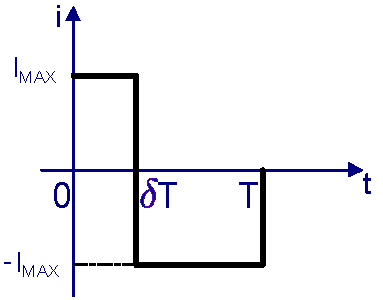
\includegraphics[width=0.7\linewidth]{current_ef_solve_3.pdf}
            \caption{ }
            \label{es:fig_current_ef_solve_3}
          \end{figure}
        
      % ===========================================================================================
      \item Výpočet efektivní hodnoty proudu s průběhem na obrázku \ref{es:fig_current_ef_solve_4}:
        \begin{figure}[ht!]
          \centering
          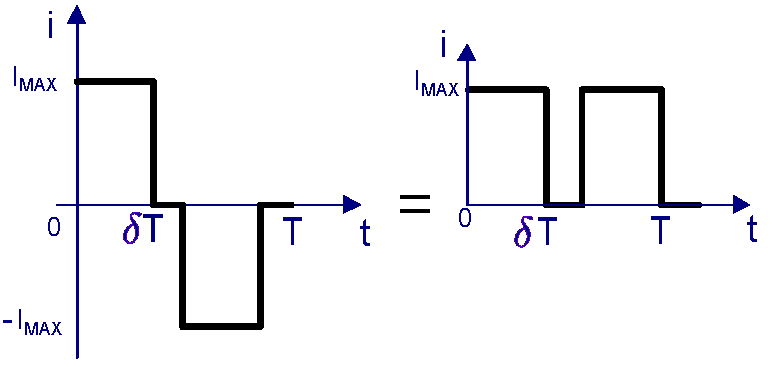
\includegraphics[width=0.9\linewidth]{current_ef_solve_4.pdf}
          \caption{$I_{ef}=I_{max}\sqrt{2\delta}$}\label{es:fig_current_ef_solve_4}
        \end{figure}
        \begin{equation}\label{es:eq_Ief4_solve}
            I_{ef}=\sqrt{I_{ef1}^2+I_{ef2}^2}=\sqrt{2I_{max}\delta}
        \end{equation}
        \begin{equation}\label{es:eq_Ief4}
            I_{ef1}^2=I_{ef2}^2=\frac{1}{T}\int_0^{\delta T}{I_{max}^2}dt
                               =\frac{1}{T}I_{max}^2[t]_0^{\delta T}=I_{max}^2\delta
        \end{equation}

      % ===========================================================================================
      \item Výpočet efektivní hodnoty proudu s průběhem na obrázku \ref{es:fig_current_ef_solve_7}:

          \begin{equation}\label{es:eq_current_ef_solve_7}
            I_{ef}^2 = \frac{1}{T}\int_0^{\delta T}{I_{max}^2}dt 
                     = \frac{1}{T}I_{max}^2[t]_0^{\delta T}=I_{max}^2\delta
          \end{equation}

          \begin{figure}
            \centering
            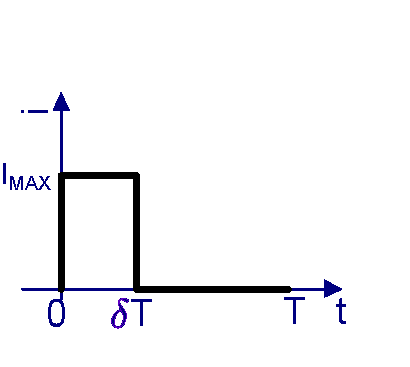
\includegraphics[width=0.8\linewidth]{current_ef_solve_7.pdf}
            \caption{ }
            \label{es:fig_current_ef_solve_7}
          \end{figure}
        
      % ===========================================================================================
      \item Výpočet efektivní hodnoty proudu s průběhem na obrázku \ref{es:fig_current_ef_solve_5}:
      
        \setlength{\parindent}{-10mm}
        \begin{minipage}[b]{0.6\textwidth}% first column 
          \begin{align*}
            I_{ef}^2 
              &=  \frac{1}{T}\int_0^{\delta T}\left(I_{max}-I_n + 
                  \frac{I_n}{\delta T}t\right)^2dt                                 \\                   
              &=  \frac{1}{T}\int_0^{\delta T}\left((I_{max}-I_n)^2t + 
                  \frac{2I_n(I_{max}-I_n)}{\delta T}t +
                 (\frac{I_n}{\delta T})^2t^2\right)dt                              \\ 
              &=  \frac{1}{T}\left((I_{max}-I_n)^2t +
                  \frac{I_n(I_{max}-I_n)}{\delta T}t^2 +
                 (\frac{I_n}{\delta T})^2\frac{t^3}{3}\right)_0^{\delta T}         \\ 
              &=  \frac{1}{T}\left((I_{max}-I_n)^2\delta T +
                  \frac{I_n(I_{max}-I_n)}{\delta T}\delta T^2 + 
                 (\frac{I_n}{\delta T})^2\frac{\delta T^3}{3}\right)               \\  
              &=  \delta\left((I_{max} - I_n)^2 + I_n\cdot(I_{max}-I_n) +
                  \frac{I_n}{3}^2\right)                                           \\  
              &=  \delta\left(I_{max}^2-2I_{max}I_n+I_{n}^2 + I_{max}I_n-I_n^2 +
                  \frac{I_n^2}{3} \right)                                          \\ 
              &=  \delta\left(I_{max}^2-I_{max}I_n+\frac{I_n^2}{3}\right)
          \end{align*}
        \end{minipage} % umožňuje použít footnote i v protstředí minipage
        \hspace{0.05\textwidth}
        \begin{minipage}[b]{0.3\textwidth}% second column
          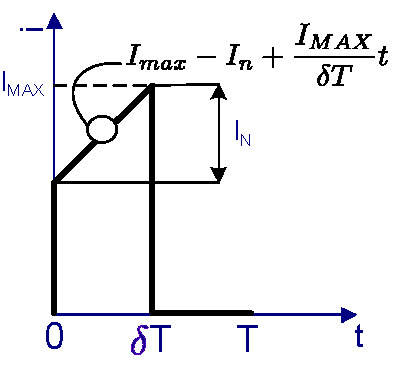
\includegraphics[width=0.9\textwidth]{current_ef_solve_5.pdf}
          \captionof{figure}{ }
          \label{es:fig_current_ef_solve_5}
        \end{minipage}\newline
        
        \begin{equation}\label{es:eq_current_ef_solve_5}
          I_{ef}=I_{max}\sqrt{\delta\left(I_{max}^2+\frac{I_n^2}{3}- I_nI_{max}\right)}
        \end{equation} 
         
      % ===========================================================================================
      \item Výpočet efektivní hodnoty proudu s průběhem na obrázku \ref{es:fig_current_ef_solve_6}:

        \setlength{\parindent}{-10mm}
        \begin{minipage}[b]{0.6\textwidth}% first column 
          \begin{align*}
            I_{ef1}^2 &=  \delta\left(I_{max}^2-I_{max}I_n+\frac{I_n^2}{3}\right)         \\
            I_{ef2}^2 &=  \frac{1}{T}\int_{\delta T}^{T(1-\delta)}\left(I_{max}
                         +\frac{I_n}{T(\delta-1)}(t-\delta T)\right)^2dt                  \\
                      &=  \text{meze:}\left(
                            \begin{array}{cc}
                                \tau = t -\delta T & \tau_h = T(1-\delta)  \\
                               d\tau = dt          & \tau_d = 0
                            \end{array}
                          \right) \\ \nonumber
                      &=  \frac{1}{T}\int_0^{T(1-\delta)}\left(I_{max} +
                          \frac{I_n}{T(\delta-1)}\tau\right)^2d\tau                       \\
                      &=  \frac{1}{T}\int_0^{T(1-\delta)}\left(I_{max}^2 +
                          \frac{2I_{max}I_n}{T(\delta-1)}\tau +
                          \left(\frac{I_n}{T(\delta-1)}\right)^2\tau^2\right)d\tau        \\
                      &=  \frac{1}{T}\left[I_{max}^2\tau +
                          \frac{I_{max}I_n}{T(\delta-1)}\tau^2 +
                          \left(\frac{I_n}{T(\delta-1)}\right)^2
                          \frac{\tau^3}{3}\right]_0^{T(1-\delta)}                         \\
                      &=  (1-\delta)\left[I_{max}^2+I_{max}I_n - \frac{I_n^2}{3}\right]
          \end{align*}
        \end{minipage} % umožňuje použít footnote i v protstředí minipage
        \hspace{0.05\textwidth}
        \begin{minipage}[b]{0.3\textwidth}% second column
          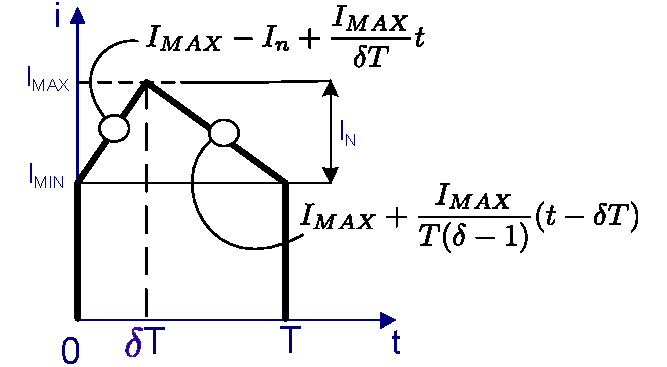
\includegraphics[width=1.2\textwidth]{current_ef_solve_6.pdf}
          \captionof{figure}{ }
          \label{es:fig_current_ef_solve_6}
        \end{minipage}\newline
        
        \begin{equation}\label{es:eq_current_ef_solve_6}
          I_{ef} = \sqrt{I_{ef1}^2+I_{ef2}^2} = \sqrt{I_{max}^2+I_{max}I_{n} - \frac{I_n^2}{3}}
        \end{equation} 

      % ===========================================================================================
      \item Výpočet efektivní hodnoty proudu s průběhem na obrázku \ref{es:fig_current_ef_solve_8}:

        \setlength{\parindent}{-10mm}
        \begin{minipage}[b]{0.6\textwidth}% first column 
          \begin{align*}
            I_{ef}^2 
              &=  \frac{1}{T}\int_0^{\delta T}{\left(I_{max}\sin(t)\right)^2}dt=
                  \frac{I_{max}^2}{T}\int_0^{\delta T}{\sin^2(t)}                                 \\ 
              &=  \frac{I_{max}^2}{T}\left[\frac{t}{2}-
                  \underbrace{\frac{\sin(t)\cos(t)}{2}}_{\sin(\delta T)=0}\right]_0^{\delta T}=
                       I_{max}^2\frac{\delta}{2}                                                  \\
          \end{align*}
        \end{minipage} % umožňuje použít footnote i v protstředí minipage
        \hspace{0.05\textwidth}
        \begin{minipage}[b]{0.3\textwidth}% second column
          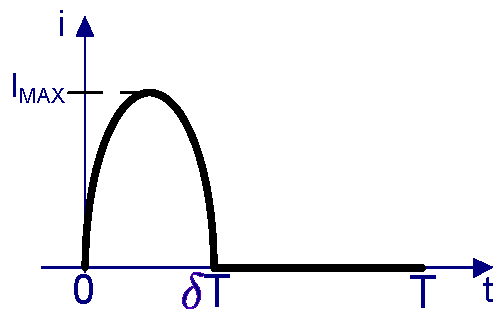
\includegraphics[width=0.9\textwidth]{current_ef_solve_8.pdf}
          \captionof{figure}{ }
          \label{es:fig_current_ef_solve_8}
        \end{minipage}\newline
        
        \begin{equation}\label{es:eq_current_ef_solve_8}
           I_{ef} = I_{max}\sqrt{\frac{\delta}{2}} 
        \end{equation} 

    \end{enumerate}

\ChapterBiblioList   